\section{Multilevel Sequentially Semiseparable P\-re\-cond\-itioning Techniques}
\label{ch:msss}
{\justify
Semiseparable matrices \cite{VV07} and the more general concept of sequentially sem\-iseparable (SSS) matrices \cite{CD05,sss_techrep03} are structured matrices represented by a set of generators. Matrices that arise from the discretization of 1D partial differential equations typically have an SSS structure~\cite{RT10}, and submatrices taken from the strict\-ly lower/upper-triangular part yield generators of low rank. Multiple applications from different areas can be found \cite{DV98,KM00,RV09aa} that exploit this structure. Multilevel sequentially sem\-iseparable (MSSS) matrices generalize SSS matrices to the case when $d>1$. Again, discretizations of higher-dimensional PDEs give rise to matrices that have an MSSS structure~\cite{QG15}, and the multilevel paradigm yields a hierarchical matrix structure with MSSS generators that are themselves MSSS of a lower hierarchical level. This way, at the lowest level, generators are SSS matrices. The advantages of Cartesian grids in higher dimensions and the resulting structure of the corresponding discretization matrices depicted in Figure \ref{fig:hier_struc} is directly exploited in MSSS matrix computations. For unstructured meshes we refer to \cite{HSS13} where hierarchically semiseparable (HSS) matrices are used. MSSS preconditioning techniques were first studied for PDE-constrained optimization problems in~\cite{QG15} and later extended to computational fluid dynamics problems~\cite{QG15a}. In this work, we apply MSSS matrix computations to precondition the time-harmonic elastic wave equation. Appropriate splitting of the 3D elastic operator leads to a sequence of 2D problems in level-2 MSSS structure. An efficient preconditioner for 2D problems is based on model order reduction of level-1 SSS matrices. 

\subsection{Definitions and basic SSS operations}
\label{ch:sss_level1}
We present the formal definition of an SSS matrix used on 1D level in Definition~\ref{def_sss}.

\begin{definition}[SSS matrix structure, \cite{CD05}]\label{def_sss}
Let $A$ be an $n \times n$ block matrix in SSS structure such that $A$ can be written in the following block-partitioned form,
\begin{equation}\label{eqn_sss_definition}
    A_{ij}=\left\{
        \begin{array}{ll}
            U_iW_{i+1}\cdots W_{j-1}V_j^\trp, & \text{if}\quad i<j, \\
            D_i, & \text{if}\quad i=j, \\
            P_iR_{i-1}\cdots R_{j+1}Q_j^\trp, & \text{if}\quad i>j.
        \end{array} 
       \right.
\end{equation}
Here, the superscript `$\trp$' denotes the conjugate transpose of a matrix. The matrices $\displaystyle \{ U_s$, $W_s$, $V_s$, $D_s$, $P_s$, $R_s$, $Q_s \}_{s=1}^n$ 
are called \textit{generators} of the SSS matrix $A$, with their respective dimensions given in Table~\ref{tab_sss_size}. As a short-hand notation for \eqref{eqn_sss_definition}, we use $A = SSS(P_s, R_s, Q_s, D_s, U_s, W_s, V_s)$.%, where $1 \leq s \leq n$.
\end{definition}
The special case of an SSS matrix when $n=4$ is presented in the appendix.
\begin{table}[ht]
\footnotesize
\centering
\caption{Generators sizes for the SSS matrix $A$ in Definition~\ref{def_sss}. Note that, for instance, $m_1+...+m_n$ equals the dimension of $A$.}\label{tab_sss_size}
\setlength{\tabcolsep}{.4em}
\begin{tabular}{ccccccc}
\hline
 $U_i$ & $W_i$ & $V_i$ & $D_i$ & $P_i$ & $R_i$ & $Q_i$ \\
\hline
 $m_i\times k_i$ & $k_{i-1}\times k_i$ & $m_i\times k_{i-1}$ & $m_i\times m_i$ & $m_i\times l_i$ & $l_{i-1}\times l_i$ & $m_i\times l_{i+1}$ \\
\hline
\end{tabular}
\end{table}

% \noindent For example, $n=4$ yields the following SSS matrix,
% \begin{equation*}%\label{eqn_sss_example}
%         A=\begin{bmatrix}
%                       D_1 & U_1V_2^\trp & U_1W_2V_3^\trp & U_1W_2W_3V_4^\trp \\
%                       P_2Q_1^\trp & D_2 & U_2V_3^\trp & U_2W_3V_4^\trp  \\
%                       P_3R_2Q_1^\trp & P_3Q_2^\trp & D_3 & U_3V_4^\trp  \\
%                       P_4R_3R_2Q_1^\trp & P_4R_3Q_2^\trp & P_4Q_3^\trp & D_4
%                     \end{bmatrix}.
% \end{equation*}

In general, every matrix can be represented in SSS format. In Figure \ref{fig:hier_struc} (bottom right) we show that the 1D level of the elastic operator is tridiagonal if $p=1$. Therefore, diagonal blocks $D_i$ are copies of the 1D operator, and off-diagonal blocks can, for instance, be represented by the product of rank-$p$ matrices, $U_2 V_3^\trp$, where the last element of $U_2$ is identical to the respective entry of the 1D operator and $V_3$ is the first unit vector. Basic operations such as addition, multiplication and inversion are closed under SSS structure and can be performed in linear computational complexity if $k_i$ and $l_i$ in Table~\ref{tab_sss_size} are bounded by a constant. The rank of the off-diagonal blocks, formally defined as the \textit{sem\-iseparable order} in Definition \ref{def_ss_order}, plays an important role in the computational complexity analysis of SSS matrix computations. 

% \begin{figure}[H]
% \centering
%   \includegraphics[width=0.4\columnwidth]{figs/13-06-52/P-crop.pdf} \hspace{0.5cm} %{figs/P31-crop.pdf} \hspace{0.5cm}
%   \includegraphics[width=0.4\columnwidth]{figs/13-06-52/P3D_orig-crop.pdf} \\ \vspace{0.5cm} %{figs/P31_x-crop.pdf} \\ \vspace{0.5cm}
%   \includegraphics[width=0.4\columnwidth]{figs/13-06-52/P2D_orig-crop.pdf} \hspace{0.5cm} %{figs/P31_xx-crop.pdf} \hspace{0.5cm}
%   \includegraphics[width=0.4\columnwidth]{figs/13-06-52/P1D_orig-crop.pdf} %{figs/P31_xx-crop.pdf} 
% \caption{A \texttt{spy} plot of a 3D problem with $p=1$. Appropriate zooming demonstrates the hierarchically repeating structure of the matrix on level 3 (top left), level 2 (top right), level 1 (bottom left), and generator level (bottom right).}
% \label{fig:hier_struc}
% \end{figure}

\begin{definition}[Semiseparable order, \cite{EG05}]\label{def_ss_order}
Let $A$ be an $n \times n$ block matrix in SSS structure satisfying Definition~\ref{def_sss}. We use a \textit{colon-style} notation: $A(i\!:\!j, k\!:\!\ell)$ selects rows of blocks from $i$ to $j$ and columns of blocks from $k$ to $\ell$ of the SSS matrix~$A$, i.e. $A(2\!:\!2,3\!:\!3) = U_2V_3^\trp$. Let
\begin{equation*}
    \text{rank}\ A(s+1\!:\!n , 1\!:\!s)=:l_s,\ s=1, 2,\ldots , n-1, \ \text{and let further,}
\end{equation*}
% and let further,
\begin{equation*}
    \text{rank}\ A(1\!:\!s , s+1\!:\!n)=:u_s,\ s=1, 2,\ldots , n-1.
\end{equation*}
Setting $r^l := \max \{l_s\}$ and $r^u := \max \{u_s\}$, we call $r^l$ the \textit{lower semiseparable order} and $r^u$ the \textit{upper semiseparable order} of $A$, respectively.
\end{definition}

If the upper and lower sem\-iseparable order are bounded by say $r^\ast$, i.e., $\{r^l,\ r^u\} \leq
r^*$, then the computational cost for the SSS matrix computations is of 
$\mathcal{O}((r^\ast)^3n)$ complexity~\cite{CD05}, where $n$ is the number of blocks of the SSS matrix as introduced in
Definition~\ref{def_sss}. We will refer to $r^\ast$ as the maximum off-diagonal rank. Matrix-matrix operations are closed under SSS
structure, but performing SSS matrix computations will increase the sem\-iseparable order, cf.~\cite{CD05}. We use model order reduction in the sense of Definition \ref{mor_sss} in order to bound the sem\-iseparable order.

Using the aforementioned definition of sem\-iseparable order, we next introduce the following lemma to compute the (exact) $LU$ factorization of an SSS matrix. 

\begin{lemma}[$LU$ factorization of an SSS matrix]\label{lu_sss}
Let $A = SSS(P_s, R_s, Q_s, D_s, U_s, W_s, V_s)$ be given in generator form with sem\-iseparable order $(r^l,\ r^u)$. Then the factors of an $LU$ factorization of $A$ are given by the following generators representation,
\begin{align*}
L &= SSS(P_s, R_s, \hat{Q}_s, D^L_s,\ 0,\ 0,\ 0), \\ 
U &= SSS(0,\ 0,\ 0,\ D_s^U, \hat{U}_s, W_s, V_s).
\end{align*}
The generators of $L$ and $U$ are computed by Algorithm~\ref{LU}. Moreover, $L$ has sem\-iseparable order $(r^l, 0)$, and $U$ has sem\-iseparable order $(0, r^u)$.
\end{lemma}
\begin{algorithm}[ht]
\caption{LU factorization and inversion of an SSS matrix $A$ \cite{sss_techrep03,VV07}}\label{LU}
% \setstretch{1.3}
\begin{algorithmic}[1]
% \Procedure{$LU$}{$A$} %\Comment{LU factorization of MSSS matrix $A$}
% \State\Require\ SSS generators of $A$ as defined in \eqref{eqn_sss_definition}
% \vspace{0.1cm}

\Procedure{INV\_SSS(A)}{} \State \parbox[t]{\dimexpr\linewidth-\algorithmicindent}{\textbf{Input:} $A = SSS(P_s, R_s, Q_s, D_s, U_s, W_s, V_s)$ in generator form\strut} 
% \State \textbf{Output:} $\left\{D_s^L\right\}_{s=1}^{n}$, $\ds \left\{D_s^U\right\}_{s=1}^{n}$, $\ds \left\{\hat{Q}_s\right\}_{s=1}^{n-1}$, $\ds \left\{\hat{U}_s\right\}_{s=1}^{n-1}$ \vspace{0.2cm}
\State // Perform LU factorization
\State $ D_1 =: D_1^L D_1^U$ \Comment{$LU$ factorization on generator level}
\State Let $\hat{U}_1:=(D_1^L)^{-1}U_1$, and $\hat{Q}_1:=( D_1^L)^{-\trp}Q_1$
\For {$i=2: n-1$}
\If {$i=2$}
\State $M_i:=\hat{Q}_{i-1}^\trp\hat{U}_{i-1}$
\Else
\State $M_i:=\hat{Q}_{i-1}^\trp\hat{U}_{i-1}+R_{i-1}M_{i-1}W_{i-1}$
\EndIf
\State $\left(D_i-P_iM_{i}V_i^\trp\right) =: D_i^L D_i^U$ \Comment{$LU$ factorization of generators}
\State Let $\hat{U}_i:=(D_i^L)^{-1}(U_i-P_iM_{i}W_i)$, and
\State let $\hat{Q}_i:=(D_i^U)^{-\trp}(Q_i-V_iM_{i}^\trp R_i^\trp)$
\EndFor
\State $M_n:=\hat{Q}_{n-1}^\trp\hat{U}_{n-1}+R_{n-1}M_{n-1}W_{n-1}$
\State $\left(D_n-P_nM_{n}V_n^\trp\right) =: D_n^L D_n^U$ \Comment{$LU$ factorization of generators}
% \State\Ensure\ $\ds \left\{D_s^L\right\}_{s=1}^{n}$, $\ds \left\{D_s^U\right\}_{s=1}^{n}$, $\ds \left\{\hat{Q}_s\right\}_{s=1}^{n-1}$, $\ds \left\{\hat{U}_s\right\}_{s=1}^{n-1}$
\State // Perform inversion
\State $L := SSS(P_s, R_s, \hat{Q}_s, D^L_s,\ 0,\ 0,\ 0)$
\State $U := SSS(0,\ 0,\ 0,\ D_s^U, \hat{U}_s, W_s, V_s)$
\State $A^{-1} = U^{-1} L^{-1}$ \Comment{SSS inversion (App. \ref{app_invsss}) \& MatMul (App. \ref{app_matmulsss})}
\EndProcedure
\end{algorithmic}
\end{algorithm}

\begin{definition}[Model order reduction of an SSS matrix]\label{mor_sss}
Let $A = SSS(P_s, R_s, Q_s, D_s, U_s, W_s, V_s)$ be an SSS matrix with lower order numbers $l_s$ and upper order numbers $u_s$. The SSS matrix $\tilde{A} = SSS(\tilde{P}_s, \tilde{R}_s, \tilde{Q}_s, D_s, \tilde{U}_s, \tilde{W}_s, \tilde{V}_s)$ is called a re\-duced order approximation of $A$, if $\| A - \tilde{A} \|_2$ is small, and for the lower and upper order numbers it holds, $\tilde{l_s} < l_s, \tilde{u_s} < u_s$ for all $1 \leq s \leq n-1$.
\end{definition}

% Algorithms for model order reduction of SSS matrices are discussed in \cite{QG15}.
\subsection{Approximate block-$LU$ decomposition using MSSS computations for 2D problems}
\label{ch:msss_lu}
Similar to Definition~\ref{def_sss} for SSS matrices, the generators representation for MSSS matrices (level-$k$ SSS matrices) is given in Definition~\ref{def_msss}.

\begin{definition}[MSSS matrix structure, \cite{QG15}]\label{def_msss}
The matrix $A$ is said to be a level-$k$ SSS matrix if it has a form like~\eqref{eqn_sss_definition} and all its 
generators are level-$(k-1)$ SSS matrices. The level-$1$ SSS matrix is the SSS matrix that satisfies Definition~\ref{def_sss} We call $A$ to be in MSSS matrix structure if $k > 1$. 
\end{definition}

Most operations for SSS matrices can directly be extended to MSSS matrix computations. In order to perform a matrix-matrix multiplication
of two MSSS matrices in linear computational complexity, model order reduction which is studied in~\cite{CD05,QG15,QG15a} is necessary to keep 
the computational complexity low. The preconditioner \eqref{eq:precon} for a 2D elastic problem is of level-$2$ MSSS structure. We present a block-$LU$ factorization of a level-2 MSSS matrix in this Section. Therefore, model order reduction is necessary which results in an \textit{approximate} block-$LU$ factorization. This approximate factorization can be used as a preconditioner for IDR($s$) in Algorithm \ref{bio_idr}. On a two-dimensional Cartesian grid, the preconditioner \eqref{eq:precon} has a $2 \times 2$ block structure as presented in Figure \ref{fig:perm} (left).

\begin{definition}[Permutation of an MSSS matrix, \cite{QG15}]\label{perm_msss}
Let $\mathcal{P}(\tau)$ be a $2 \times 2$ level-2 MSSS block matrix arising from the FEM discretization of \eqref{eq:precon} using linear B-splines ($p=1$),
\begin{equation}
\label{eq:L2Msss}
 \mathcal{P}(\tau) = \begin{bmatrix}
                      \mathcal{P}_{11} & \mathcal{P}_{12}\\
                      \mathcal{P}_{21} & \mathcal{P}_{22}\\
                     \end{bmatrix} \in \mathbb{C}^{2n_xn_y \times 2n_xn_y},
\end{equation}
 with block entries being level-2 MSSS matrices in generator form,
\begin{align}
 \mathcal{P}_{11} &= MSSS(P_s^{11}, R_s^{11}, Q_s^{11}, D_s^{11}, U_s^{11}, W_s^{11}, V_s^{11}), \tag{16a} \label{P11gen}\\
 \mathcal{P}_{12} &= MSSS(P_s^{12}, R_s^{12}, Q_s^{12}, D_s^{12}, U_s^{12}, W_s^{12}, V_s^{12}), \tag{16b} \label{P12gen}\\
 \mathcal{P}_{21} &= MSSS(P_s^{21}, R_s^{21}, Q_s^{21}, D_s^{21}, U_s^{21}, W_s^{21}, V_s^{21}), \tag{16c} \label{P21gen}\\
 \mathcal{P}_{22} &= MSSS(P_s^{22}, R_s^{22}, Q_s^{22}, D_s^{22}, U_s^{22}, W_s^{22}, V_s^{22}), \tag{16d} \label{P22gen} \setcounter{equation}{16}
\end{align}
where $1 \leq s \leq n_x$. Note that all generators in \eqref{P11gen}-\eqref{P22gen} are SSS matrices of (fixed) dimension $n_y$. Let $\{m_s\}_{s=1}^{n}$ be the dimensions of the diagonal generators of such an SSS matrix, cf. \mbox{Table \ref{tab_sss_size}}, with $\sum_{s=1}^n m_s = n_y$. Then there exists a permutation matrix $\Psi$, $\Psi \Psi^\mathsf{T} = \Psi^\mathsf{T} \Psi = I$, given by
\begin{align}
\label{eq:Psi}
\Psi = \left[ I_{n_x} \otimes \begin{bmatrix} \Psi_{1D} \\ 0 \end{bmatrix} \quad I_{n_x} \otimes \begin{bmatrix} 0 \\ \Psi_{1D} \end{bmatrix} \right],
\end{align}
where
\begin{align*}
\Psi_{1D} := \left[ \text{blkdiag}\left( \begin{bmatrix} I_{m_s} \\ 0 \end{bmatrix} \right)_{s=1}^n \quad \text{blkdiag}\left( \begin{bmatrix} 0 \\I_{m_s} \end{bmatrix} \right)_{s=1}^n \right],
\end{align*}
% where
% \begin{align*}
% \Psi = \left[ \text{blkdiag}\left( \begin{bmatrix} I_{m_s^{11}} \\ 0 \end{bmatrix} \right)_{s=1}^n \quad \text{blkdiag}\left( \begin{bmatrix} 0 \\I_{m_s^{22}} \end{bmatrix} \right)_{s=1}^n \right]
% \end{align*}
such that $\mathcal{P}_{2D}(\tau) = \Psi^\mathsf{T} \mathcal{P}(\tau) \Psi$ is of global MSSS level-2 structure.
\end{definition}

We illustrate the effect of the permutation matrix $\Psi$ in Figure \ref{fig:perm}. For a matrix \eqref{eq:precon} that results from a discretization of the 2D time-harmonic elastic wave equation, $P_{2D}$ is of block tri-diagonal MSSS structure.

\begin{corollary}[Block tri-diagonal permutation]\label{tri_perm}
Consider in Definition \ref{perm_msss} the special case that the block entries in \eqref{eq:L2Msss} are given as,
\begin{align}
 \mathcal{P}_{11} &= MSSS(P_s^{11}, 0, \underbar{I}, D_s^{11}, U_s^{11}, 0, \underbar{I}), \tag{18a} \label{P11}\\
 \mathcal{P}_{12} &= MSSS(P_s^{12}, 0, \underbar{I}, D_s^{12}, U_s^{12}, 0, \underbar{I}), \tag{18b} \label{P12}\\
 \mathcal{P}_{21} &= MSSS(P_s^{21}, 0, \underbar{I}, D_s^{21}, U_s^{21}, 0, \underbar{I}), \tag{18c} \label{P21}\\
 \mathcal{P}_{22} &= MSSS(P_s^{22}, 0, \underbar{I}, D_s^{22}, U_s^{22}, 0, \underbar{I}), \tag{18d} \label{P22} \setcounter{equation}{18}
\end{align}
with rectangular matrix $\underbar{I} = [I,0]$. Then the matrix $\Psi^\mathsf{T} \mathcal{P}(\tau) \Psi$ is of block tri-diagonal MSSS structure.
\end{corollary}
\begin{proof}
 This result follows from formula (2.13) of Lemma 2.4 in the original proof \cite{QG15} when generators $R^{ij}_s=W^{ij}_s\equiv0$ for $ i,j \in \{1,2\}$. \qed
\end{proof}

\begin{figure}[H]
\centering
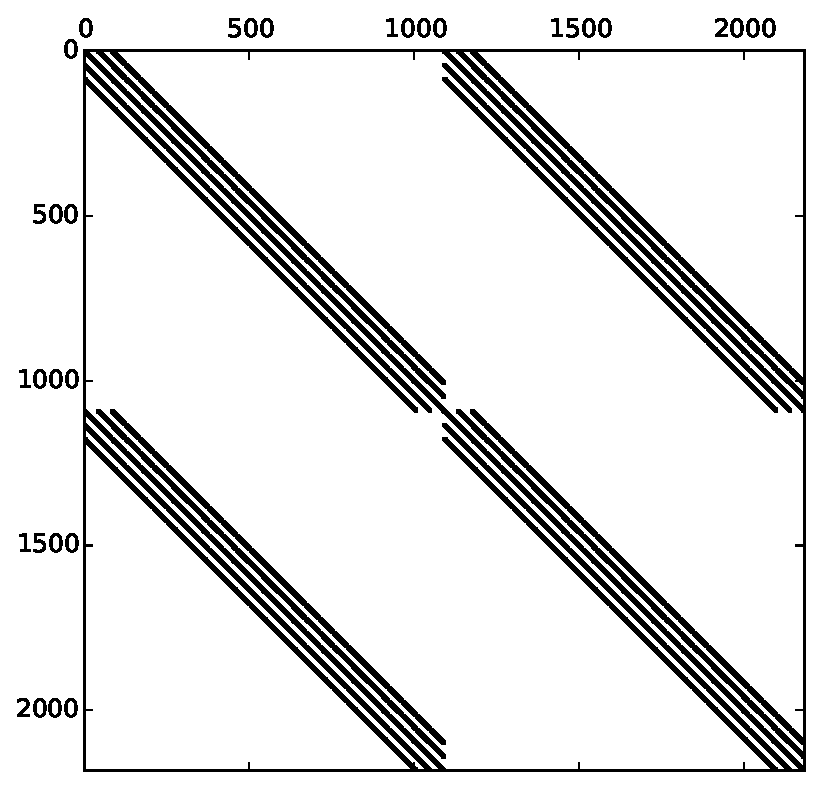
\includegraphics[width=0.49\columnwidth]{P_25_25-crop} \hfill
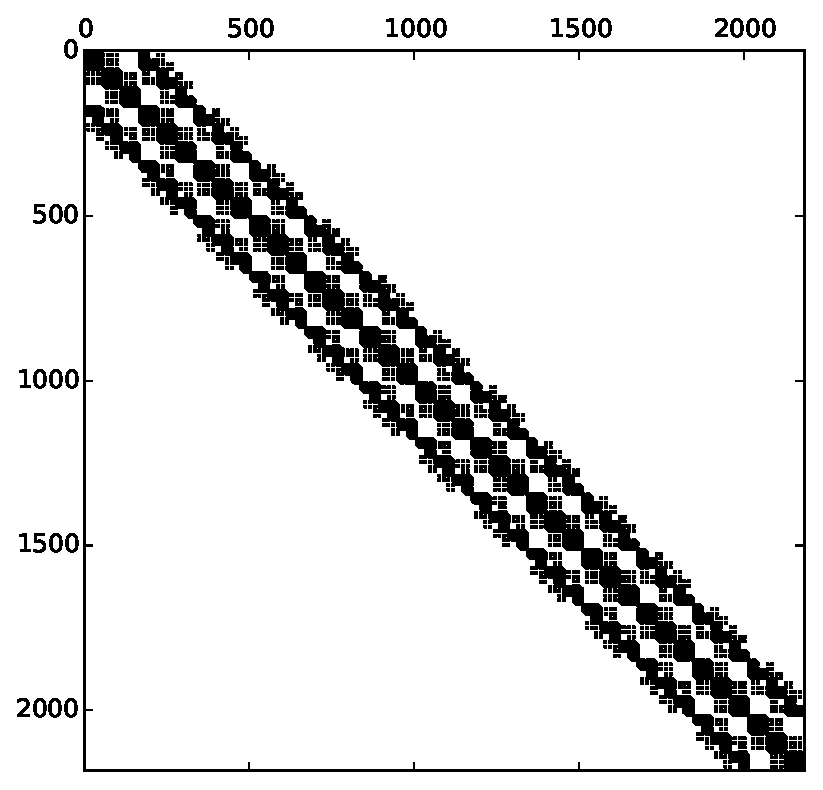
\includegraphics[width=0.49\columnwidth]{P_25_25_perm-crop}
\caption{A \texttt{spy} plot of $\mathcal{P}(\tau)$ for the \texttt{wedge} problem (left) and $\Psi^\mathsf{T} \mathcal{P}(\tau) \Psi$ (right) for $d=p=2$, and \texttt{nnz=100,587} in both cases. Clearly, the permutation leads to a reduction in bandwidth, and the permuted matrix is block tri-diagonal.}
\label{fig:perm}
\end{figure}

If the matrix \eqref{eq:L2Msss} is sparse, it is advisable to use a sparse data structure on generator-level for \eqref{P11}-\eqref{P22} as well. Because of Corollary \ref{tri_perm}, the permuted 2D preconditioner can be written as,
\begin{equation}
\label{eq:perm_precon}
         \mathcal{P}_{2D}= \Psi^\mathsf{T} \mathcal{P}(\tau) \Psi =\begin{bmatrix}
                     P_{1,1} & P_{1,2} &         &        \\
                     P_{2,1} & P_{2,2} & P_{2,3} &        \\
%                              & P_{3,2} & P_{3,3} & \ddots & \\
                                     & \ddots  & \ddots & \ddots \\
                                     &         & \ddots & P_{n_x, n_x}
                 \end{bmatrix}
\end{equation}
with block entries $P_{i,j}$ in SSS format according to \mbox{Definition \ref{def_sss}}, compare Figure \ref{fig:perm} (right). We perform a block-LU factorization of the form $\mathcal{P}_{2D} = L S U$, with 
\begin{equation}
\label{eq:full_Schur}
        L_{i,j}=\begin{cases}
             I &\hspace{-0.2cm} \text{if}\ i=j \\
             P_{i,j}S_j^{-1} &\hspace{-0.2cm} \text{if}\ i = j+1
	     \end{cases}, \
	U_{i,j}=\begin{cases}
             I &\hspace{-0.2cm} \text{if}\ j=i \\
             S_i^{-1}P_{i,j} &\hspace{-0.2cm} \text{if}\ j = i+1
	     \end{cases},     
\end{equation}
and Schur complements given by
\begin{equation}\label{eqn_schur}
        S_i=\begin{cases}
             P_{i,i} & \text{if}\ i=1 \\
             P_{i,i}-P_{i,i-1}S_{i-1}^{-1}P_{i-1,i} & \text{if}\ 2\leq i\leq n_x.
	     \end{cases}
\end{equation}

The Schur complements in \eqref{eq:full_Schur}-\eqref{eqn_schur} are SSS matrices and inverses can be computed with Algorithm \ref{LU}. From Lem\-ma \ref{lu_sss}, we conclude that this does not increase the respective off-diagonal ranks. However, in \eqref{eq:full_Schur}-\eqref{eqn_schur}, we also need to perform matrix-matrix multiplications and additions of SSS matrices which lead to an increase in rank, cf. \cite{CD05} and Appendix \ref{app_matmulsss}. Therefore, we apply model order reduction in the sense of Definition \ref{mor_sss} at each step $i$ of the recursion \eqref{eqn_schur} in order to limit the off-diagonal rank. An algorithm that limits the off-diagonal ranks to a constant, say $r^\ast$, can be found in \cite{QG15}. This leads to approximate Schur complements and, hence, an inexact $LU$ factorization. In Experiment \ref{exp:off_rank}, we show that for small off-diagonal ranks this approach results in a very good preconditioner for 2D elastic problems.

\subsection{SSOR splitting using MSSS computations for 3D problems}
\label{ch_msss3d}
For 3D problems, we consider a nodal-based FEM discretization of \eqref{eq:precon} with $n_z$ being the outermost dimension, as shown in Figure \ref{fig:precon3d} for different order of B-splines. In order to derive a memory-efficient algorithm for 3D problems, we consider the matrix splitting,
\begin{align}
\label{eq:splitting}
\mathcal{P}_{3D}(\tau) = \underbar{L} + \hat{S} + \overbar{U}, \quad \hat{S} = \text{blkdiag}(\hat{S}_1,...,\hat{S}_{n_z}),
\end{align}
where $\underbar{L}$ and $\overbar{U}$ are the (sparse) strictly lower and strictly upper parts of $\mathcal{P}_{3D}(\tau)$, and $\hat{S}$ is a block-diagonal matrix with blocks $\hat{S}_i$ being in level-2 MSSS structure. This data structure is illustrated in Figure \ref{L3scheme}.

 \begin{figure}[ht]
     \centering
     \begin{subfigure}{0.31\columnwidth}
         \centering
         \includegraphics[width=\textwidth]{P3d_p1-crop_small.pdf}%{figs/P3d_p1-crop.pdf}
         \caption{$p=1$}
     \end{subfigure}%
     ~ 
     \begin{subfigure}{0.31\columnwidth}
         \centering
         \includegraphics[width=\textwidth]{P3d_p2-crop_small.pdf}%{figs/P3d_p2-crop.pdf}
         \caption{$p=2$}
     \end{subfigure}
     ~ 
     \begin{subfigure}{0.31\columnwidth}
         \centering
 	\includegraphics[width=\textwidth]{P3d_p3-crop_small.pdf}%{figs/P3d_p3-crop.pdf}
         \caption{$p=3$}
     \end{subfigure}
     \caption{Nodal-based discretization of $\mathcal{P}_{3D}(\tau)$ in 3D for different degrees $p$ of FEM basis function.} \label{fig:precon3d}
 \end{figure}
According to \cite[Section 4.1.2]{S03}, the SSOR preconditioner based on the splitting \eqref{eq:splitting} is given by,
\begin{align*}
\mathcal{P}_{3D}(\tau) = \frac{1}{\ssorfac(2-\ssorfac)}(\ssorfac\ \underbar{L}+\hat{S}) \hat{S}^{-1} (\ssorfac\ \overbar{U}+\hat{S})
\end{align*}
which for $\ssorfac=1$ equals,
\begin{align}
\label{eq:approx_Schur}
\mathcal{P}_{3D}(\tau) = (\underbar{L}\hat{S}^{-1} + I) \hat{S} (\hat{S}^{-1}\overbar{U} + I).
\end{align}
In \eqref{eq:approx_Schur} we note that this decomposition coincides with the 2D approach \eqref{eq:full_Schur}-\eqref{eqn_schur} when the term ``$P_{i,i-1}S_{i-1}^{-1}P_{i-1,i}$'' in the Schur complements \eqref{eqn_schur} is neglected. This choice avoids a rank increase due to multiplication and addition, but yields a \textit{worse} preconditioner than in 2D. The block entries $\hat{S}_i$ ,$i=1,..,n_z$, are in level-2 MSSS structure and, hence, formula \eqref{eq:full_Schur}-\eqref{eqn_schur} can be applied sequentially for the inverses that appear in \eqref{eq:approx_Schur}. In order to invert level-1 SSS matrices that recursively appear in \eqref{eqn_schur}, we use Algorithm \ref{LU}. On the generator level, we use suitable \texttt{LAPACK} routines; cf. Table \ref{tab:algorithms} for an overview of the different algorithms used at each level.
\begin{table}[H]
\centering
\caption{Overview of algorithms applied at different levels for the (approximate) inversion of the preconditioner \eqref{eq:approx_Schur}.}\label{tab:algorithms}
\begin{tabular}{|c|c|c|}
 \hline
 \textbf{level} & \textbf{algorithm for} $\mathbf{(\cdot)^{-1}}$& \textbf{datatype} \\
 \hline
 3D MSSS& SSOR decomposition \eqref{eq:approx_Schur} & \texttt{sparse} + \texttt{L2\_SSS}\\
 2D MSSS & Schur \eqref{eq:full_Schur}-\eqref{eqn_schur} \& MOR & \texttt{tridiag. L2\_SSS} \\
 1D SSS\phantom{M}& Algorithm \ref{LU} & \texttt{L1\_SSS} \eqref{eqn_sss_definition}\\
 generator & \texttt{LAPACK} routines & set of sparse matrices\\
 \hline
\end{tabular}
\end{table}

We illustrate the data structure of the preconditioner \eqref{eq:approx_Schur} in 3D for the case of linear B-splines ($p=1$) in Figure \ref{fig:datastruc}. On level-3, we use a mixed data format that is most memory-efficient for the splitting \eqref{eq:splitting}. Since only diagonal blocks need to be inverted, we convert those to level-2 MSSS format, and keep the off-diagonal blocks of $\underbar{L}$ and $\overbar{U}$ in sparse format.
\begin{figure}[ht]
    \centering
    \begin{subfigure}{0.3\columnwidth}
        \centering
        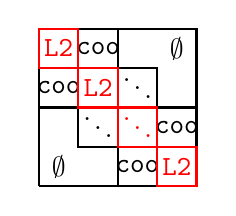
\begin{tikzpicture}
              
          \draw[black,thick] (0.5,2) -- (0.5,1.5) --(1,1.5) -- (1,2) -- (0.5,2);
          \node at (0.75,1.75) {\color{black}{\texttt{coo}}};
          
          \draw[black,thick] (0,1.5) -- (0,1) --(0.5,1) -- (0.5,1.5) -- (0,1.5);
          \node at (0.25,1.25) {\color{black}{\texttt{coo}}};
          
           \draw[black,thick] (0.5,1) -- (0.5,0.5) --(1,0.5) -- (1,1) -- (0.5,1);
           \node at (0.75,0.85) {\color{black}{$\ddots$}};
          
           \draw[black,thick] (1,0.5) -- (1,0) --(1.5,0) -- (1.5,0.5) -- (1,0.5);
           \node at (1.25,0.25) {\color{black}{\texttt{coo}}};
           
           \draw[black,thick] (1,1.5) -- (1,1) --(1.5,1) -- (1.5,1.5) -- (1,1.5);
           \node at (1.25,1.35) {\color{black}{$\ddots$}};
           
           \draw[black,thick] (1.5,1) -- (1.5,0.5) --(2,0.5) -- (2,1) -- (1.5,1);
           \node at (1.75,0.75) {\color{black}{\texttt{coo}}};

           
           \draw[thick] (0,0) -- (2,0) -- (2,2) -- (0,2) -- (0,0);
          
           
          \draw[red,thick] (0,2) -- (0,1.5) --(0.5,1.5) -- (0.5,2.0) -- cycle;
          \node at (0.25,1.75) {\color{red}{\texttt{L2}}};
          
          \draw[red,thick] (0.5,1.5) -- (0.5,1) --(1,1) -- (1,1.5) -- (0.5,1.5);
          \node at (0.75,1.25) {\color{red}{\texttt{L2}}};
          
          \draw[red,thick] (1,1) -- (1,0.5) --(1.5,0.5) -- (1.5,1) -- (1,1);
          \node at (1.25,0.85) {$\color{red}{\ddots}$};

          \draw[red,thick] (1.5,0.5) -- (1.5,0) --(2,0) -- (2,0.5) -- (1.5,0.5);
          \node at (1.75,0.25) {\color{red}{\texttt{L2}}};
          
          \node at (0.25,0.25) {$\emptyset$};
          \node at (1.75,1.75) {$\emptyset$};
          
          
%           \draw[red,thick,overlay,->] (0.25,2) to [bend left=35] (2.75,2);
          
        \end{tikzpicture}
        \caption{\texttt{L3\_SSS}}\label{L3scheme}
    \end{subfigure}%
    ~ 
    \begin{subfigure}{0.3\columnwidth}
        \centering
         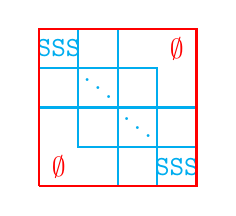
\begin{tikzpicture} 
                   
          \draw[cyan,thick] (0,2) -- (0,1.5) --(0.5,1.5) -- (0.5,2.0) -- (0,2);
          \node at (0.25,1.75) {\color{cyan}{\texttt{SSS}}};
          
          \draw[cyan,thick] (0.5,1.5) -- (0.5,1) --(1,1) -- (1,1.5) -- (0.5,1.5);
          \node at (0.75,1.35) {$\color{cyan}{\ddots}$};
          
          \draw[cyan,thick] (1,1) -- (1,0.5) --(1.5,0.5) -- (1.5,1) -- (1,1);
          \node at (1.25,0.85) {$\color{cyan}{\ddots}$};

          \draw[cyan,thick] (1.5,0.5) -- (1.5,0) --(2,0) -- (2,0.5) -- (1.5,0.5);
          \node at (1.75,0.25) {\color{cyan}{\texttt{SSS}}};
                   
          
          \draw[cyan,thick] (0.5,2) -- (0.5,1.5) --(1,1.5) -- (1,2) -- (0.5,2);
%           \node at (0.75,1.75) {\color{cyan}{\texttt{SSS}}};
          
          \draw[cyan,thick] (0,1.5) -- (0,1) --(0.5,1) -- (0.5,1.5) -- (0,1.5);
%           \node at (0.25,1.25) {\color{cyan}{\texttt{SSS}}};
          
          \draw[cyan,thick] (0.5,1) -- (0.5,0.5) --(1,0.5) -- (1,1) -- (0.5,1);
%           \node at (0.25,1.25) {\color{cyan}{\texttt{SSS}}};
          
           \draw[cyan,thick] (1,0.5) -- (1,0) --(1.5,0) -- (1.5,0.5) -- (1,0.5);
%           \node at (0.25,1.25) {\color{cyan}{\texttt{SSS}}};

           \draw[cyan,thick] (1,1.5) -- (1,1) --(1.5,1) -- (1.5,1.5) -- (1,1.5);
%           \node at (0.25,1.25) {\color{cyan}{\texttt{SSS}}};

           \draw[cyan,thick] (1.5,1) -- (1.5,0.5) --(2,0.5) -- (2,1) -- (1.5,1);
%           \node at (0.25,1.25) {\color{cyan}{\texttt{SSS}}};
          
          
          \node at (0.25,0.25) {$\color{red}{\emptyset}$};
          \node at (1.75,1.75) {$\color{red}{\emptyset}$};
          
          \draw[red, thick] (0,0) -- (2,0) -- (2,2) -- (0,2) -- (0,0);
        \end{tikzpicture}
        \caption{\texttt{L2\_SSS}, def. \ref{def_msss}}\label{L2scheme}
    \end{subfigure}
    ~ 
    \begin{subfigure}{0.3\columnwidth}
        \centering
         \begin{tikzpicture}
          
          \draw[dimgray,thick] (0.5,2) -- (0.5,1.5) --(1,1.5) -- (1,2) -- (0.5,2);
          \node at (0.75,1.75) {\tiny{$\color{dimgray}{U_1 V_2^\trp}$}};
          
           \draw[dimgray,thick] (1,1.5) -- (1,1) --(1.5,1) -- (1.5,1.5) -- (1,1.5);      
           \node at (1.25,1.35) {$\color{dimgray}{\ddots}$};
           
           \draw[dimgray,thick] (1.5,1) -- (1.5,0.5) --(2,0.5) -- (2,1) -- (1.5,1);
%            \node at (1.75,0.85) {$\color{dimgray}{\ddots}$};
           
           \draw[dimgray,thick] (1,0.5) -- (1,0) --(1.5,0) -- (1.5,0.5) -- (1,0.5);
%            \node at (1.25,0.35)  {$\color{dimgray}{\ddots}$};
           
           \draw[dimgray,thick] (0,1.5) -- (0,1) --(0.5,1) -- (0.5,1.5) -- (0,1.5);
          \node at (0.25,1.25) {\tiny{$\color{dimgray}{P_2 Q_1^\trp}$}};
          
           \draw[dimgray,thick] (0.5,1) -- (0.5,0.5) --(1,0.5) -- (1,1) -- (0.5,1);
           \node at (0.75,0.85) {\color{dimgray}{$\ddots$}};
          
           \draw[dimgray,thick] (0,0.5) -- (0.5,0.5);
           \draw[dimgray,thick] (0.5,0.5) -- (0.5,0);
           
           \draw[dimgray,thick] (1.5,2) -- (1.5,1.5);
           \draw[dimgray,thick] (1.5,1.5) -- (2,1.5);
           
           \node at (1.25,1.75) {$\color{dimgray}{\hdots}$};
           \node at (0.25,0.85) {$\color{dimgray}{\vdots}$};
           
          
          \draw[black,thick] (0,2) -- (0,1.5) --(0.5,1.5) -- (0.5,2.0) -- (0,2);
          \node at (0.25,1.75) {$\color{black}{D_1}$};
          
          \draw[black,thick] (0.5,1.5) -- (0.5,1) --(1,1) -- (1,1.5) -- (0.5,1.5);
          \node at (0.75,1.25) {$\color{black}{D_2}$};
          
          \draw[black,thick] (1,1) -- (1,0.5) --(1.5,0.5) -- (1.5,1) -- (1,1);
          \node at (1.25,0.85) {$\color{black}{\ddots}$};

          \draw[black,thick] (1.5,0.5) -- (1.5,0) --(2,0) -- (2,0.5) -- (1.5,0.5);
          \node at (1.75,0.25) {$\color{black}{D_n}$};
          
          
          \draw[cyan, thick] (0,0) -- (2,0) -- (2,2) -- (0,2) -- (0,0);
    
          
        \end{tikzpicture}
        \caption{\texttt{SSS}, def. \ref{def_sss}}\label{L1scheme}
    \end{subfigure}
    \caption{Nested data structure for the preconditioner \eqref{eq:perm_precon} after permutation for $d=3$ and $p = 1$. With \texttt{'coo'} we abbreviate the coordinate-based sparse data structure as used, for instance, in \cite{sparsekit}.}\label{fig:datastruc}
\end{figure}

For $p>1$, we apply the permutation of Definition \ref{perm_msss} on each diagonal block of $\hat S$, cf. Figure \ref{fig:precon3d_level2}. This way, the Schur decomposition described in Section \ref{ch:msss_lu} can be applied for inverting block tri-diagonal level-2 MSSS matrices.
\begin{figure}[ht]
    \centering
    \begin{subfigure}{0.45\columnwidth}
        \centering
        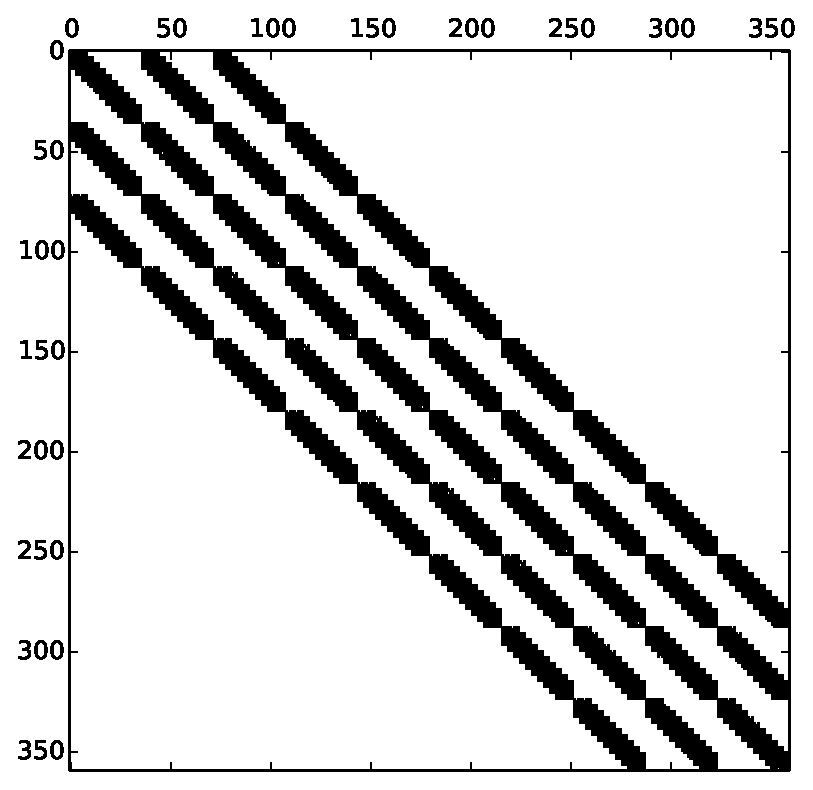
\includegraphics[width=\textwidth]{Si_p2-crop}
        \caption{$\hat{S}_i, \ 1 \leq i \leq n_x$}
    \end{subfigure}%
    ~ \hfill
    \begin{subfigure}{0.45\columnwidth}
        \centering
        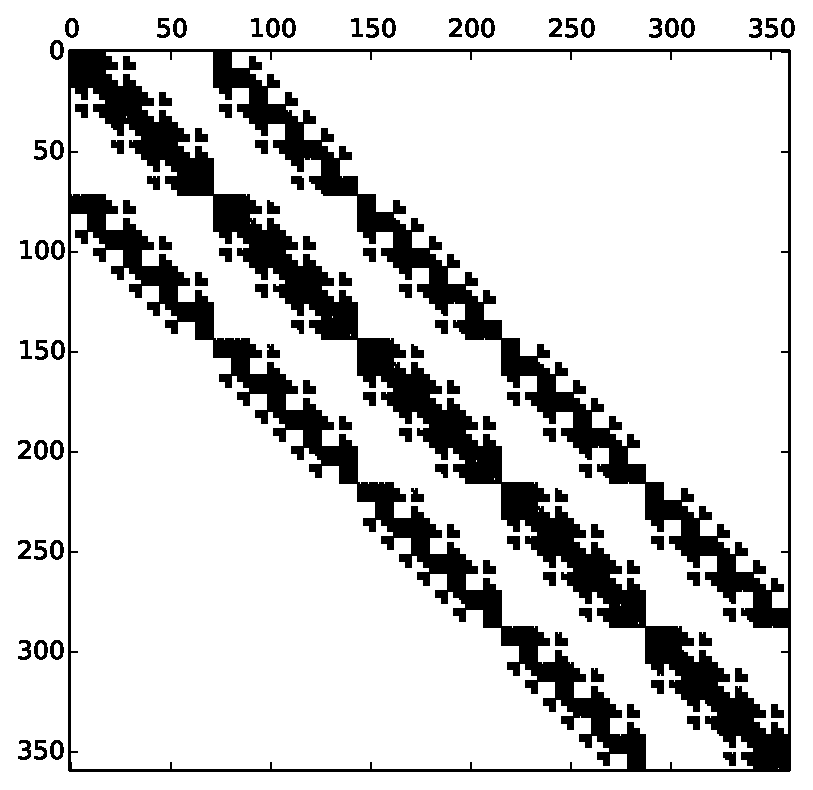
\includegraphics[width=\textwidth]{Si_p2_perm-crop}
        \caption{$\Psi^\mathsf{T} \hat{S}_i \Psi$}
    \end{subfigure}

    \caption{Permutation on level-2 leads to a block tri-diagonal level-2 MSSS matrix for $p>1$.} \label{fig:precon3d_level2}
\end{figure}

\subsection{Memory analysis for 2D and 3D MSSS preconditioner}
We finish our description of MSSS preconditioners with a memory analysis of the suggested algorithms described for 2D problems in Section \ref{ch:msss_lu}, and for 3D problems in Section \ref{ch_msss3d}, respectively. The following Corollary \ref{mem_3d} shows that in both cases we obtain linear memory requirements in terms of the problem size \eqref{eq:unknows}.
\begin{figure}[ht]
    \centering
    \begin{tikzpicture}
     \node at (0,0) {\includegraphics[scale=0.2]{z_planes2.png}};
     \node at (-1.3,1.3)  {${\color{white}\mathbf{\hat{S}_1}}$};
     \node at (-1.18,0.7)  {${\color{white}\mathbf{\hat{S}_2}}$};
     \node at (-1.01,0.04) {${\color{white}\mathbf{\hat{S}_3}}$};
     
     \node at (-0.6,-1.65) {${\color{white}\mathbf{\hat{S}_{n_z}}}$};
     
     \draw [->] (-2.4,1.0) -- (-2.15,-0.1);
     \node at (-2.55,0.7) {$z$};
    \end{tikzpicture}
    \caption{Schematic illustration: The diagonal blocks of $\hat{S}$ in \eqref{eq:splitting} correspond to a sequence of $n_z$ 2D problems in the $xy-$plane.} \label{fig:3dscheme}
\end{figure}
\begin{corollary}[Linear memory requirement]\label{mem_3d}
Consider \mbox{$p=1$} and a three-dimensional problem of size $n_x \times n_y \times n_z$. For simplicity, we assume on the generator-level $m_i \equiv m$, and the off-diagonal ranks of the inverse Schur complements $S_i$ in \eqref{eqn_schur} being limited by $k_i = l_i\equiv r^\ast$. The grid size in $y$-direction on level-1 implies $n$ generators via $n = d n_y m^{-1}$, with $m$ being a constant and $d \in \{2,3\}$. The memory requirement of the preconditioners $\mathcal{P}_{2D}$ and $\mathcal{P}_{3D}$ presented in Section \ref{ch:msss_lu} and Section \ref{ch_msss3d}, respectively, is linear in the respective problem dimension \eqref{eq:unknows}.
\end{corollary}
\begin{proof}
Consider the preconditioner $\mathcal{P}_{2D}=LSU$ given by \eqref{eq:full_Schur}-\eqref{eqn_schur}. Besides blocks of the original operator, an additional storage of $n_x$ inverse Schur complements $S_i^{-1}$ in SSS format is required,
\begin{align*}
 \texttt{mem}(\mathcal{P}_{2D}^{-1},r^\ast) &= \texttt{mem}(\mathcal{P}_{2D})  + \sum_{i=1}^{n_x} \texttt{mem}(S_{i}^{-1},r^\ast) \in \mathcal{O}(n_xn_y).
\end{align*}
The approximate Schur decomposition described in Section \ref{ch:msss_lu} allows dense, full rank diagonal generators $D_i, 1 \leq i \leq n,$ of size $m \times m$, and limits the rank of all off-diagonal generators by $r^\ast$ using model order reduction techniques:
\begin{align*}
\texttt{mem}(S_{i}^{-1},r^\ast) = \underbrace{n \cdot m^2}_{\sim D_i} + \underbrace{4(n-1)mr^\ast}_{\sim \{U_i,V_i,P_i,Q_i\}} + \underbrace{2(n-2)r^\ast r^\ast}_{\sim \{W_i,R_i\}} \in \mathcal{O}(n_y).
\end{align*}
Concerning the memory requirement for storing $\mathcal{P}_{2D}$ in MSSS format, we first note that the permutation described in Corollary \ref{tri_perm} does not affect the memory consumption. Since we use sparse generators in \eqref{P11}-\eqref{P22}, the memory requirement is of the same order as the original, sparse matrix \eqref{eq:precon} obtained from the FEM discretization.

For 3D problems, we suggest the usage of $\mathcal{P}_{3D}$ as in \eqref{eq:approx_Schur} based on the splitting \eqref{eq:splitting}. For the data structure, we keep the strictly lower and upper diagonal parts in sparse format and convert the diagonal blocks to level-2 MSSS format, cf. Figure \ref{fig:3dscheme},
\begin{align*}
 \texttt{mem}(\mathcal{P}_{3D}^{-1},r^\ast) &=  n_z \cdot \texttt{mem}(\mathcal{P}_{2D}^{-1},r^\ast) + \texttt{nnz}(\underbar{L}) + \texttt{nnz}(\overbar{U}) \\ &\in \mathcal{O}(n_xn_yn_z).
\end{align*}
\qed
\end{proof}
Note that the case $p>1$ also yields a linear memory requirement but is, for simplicity, not addressed here.
